%% LaTeX2e class for student theses
%% sections/content.tex
%%
%% Karlsruhe University of Applied Sciences
%% Faculty of  Computer Science and Business Information Systems
%% Distributed Systems (vsys)
%%
%% Prof. Dr. Christian Zirpins
%% christian.zirpins@hs-karlsruhe.de
%%
%%
%% Version 0.2, 2017-11-15
%%
%% --------------------------------------------------------
%% | Derived from sdqthesis by Erik Burger burger@kit.edu |
%% --------------------------------------------------------

\chapter{Implementierung eines ActivityPub Prototyps}
Die IDataSource Implementierung wird für das Unternehmen angefertigt in der die Bachelor Thesis bearbeitet wird. Im Falle man möchte den Service mit einer anderen Datenquelle versorgen, kann das IDataSource Interface implementiert und so angepasst werden, dass eine andere Datenbank Verwendung findet.\\
\begin{figure}[h]
	\begin{minipage}{\textwidth}
		\centering
		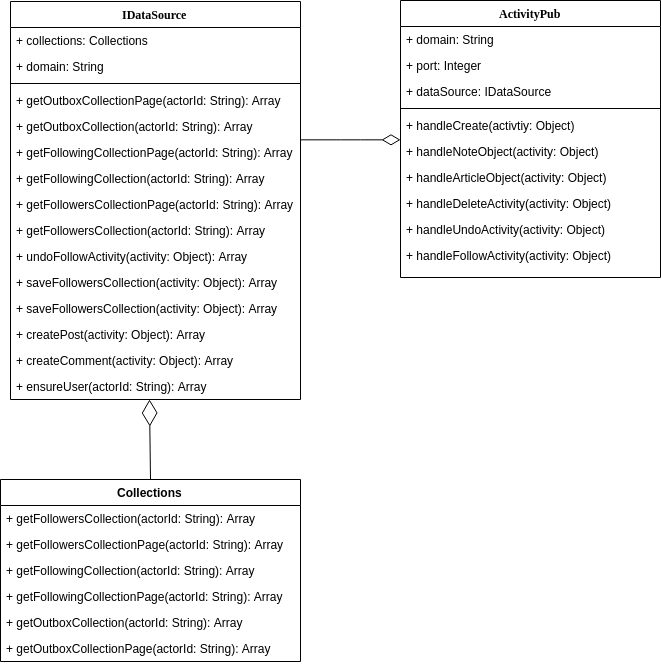
\includegraphics[scale=0.6]{figures/klassendiagramm-activitypub.png}
		\label{klassendiagramm-activitypub}
		\caption{Hauptkomponenten des förderierten Servers}
	\end{minipage}
\end{figure}
Obig abgebildetes Klassendiagramm zeigt die Hauptkomponenten des ActivityPub Services und die enthaltenen Methoden.\\

Die \glqq Collections\grqq~Klasse ist eine Fassaden Klasse und enthält Methoden die auf das IDataSource Interface zugreifen um folgende Sammlungen zu erhalten:
\begin{itemize}
	\item Followers Collection
	\item Following Collection
	\item Outbox Collection
\end{itemize} 
Sie dient ausschließlich der Lesbarkeit für den Entwickler.\\

Bei der ActivityPub Klasse handelt es sich um den Eingangspunkt. Die entsprechenden Anfrage-Handler wandeln die Anfrage in einen Service Aufruf um. Diese Klasse enthält nicht nur Handler für eingehende, sondern auch Methoden zum senden von Anfragen.\\

Für eine Integration in verschiedenste Applikationen wurden alle Datenbankspezifischen Methoden in das \textit{IDataSource} Interface ausgelagert. Durch die Implementierung dieses Interfaces können Aktivitäten ActivityPub konform empfangen werden. Das senden wiederum muss jedes Backend selbst implementieren. Dafür stehen in der ActivityPub Klasse Methoden zum senden von Aktivitäten bereit. Durch importieren der ActivityPub Klasse erhält man eine Instanz, worüber die Methoden verfügbar sind. Zum senden werden die Daten in eine Aktivität verpackt, was über die Nutzung einer \gls{as2} Bibliothek geschehen kann oder durch Erstellung mit Objekt Literalen. Bei letztere Variante muss sich zusätzlich um Kontexte und weiteres gekümmert werden.\\

Die Datenquelle kann durch die Nutzung von Datenbanken und \glq{api}'s ausgewechselt werden. Es kann eine relationale oder auch nicht-relationale Datenbank, wie z. B. MySQL oder MongoDB, genutzt werden. Bei der Prototyp Implementierung in dieser Bachelor Arbeit wird eine GraphQL Schnittstelle angesprochen.\\

Im \glqq utils\grqq~Ordner befinden sich verschiedene Dateien welche Funktionen mit dem Namen entsprechender Funktionalität exportieren um dies zu bewerkstelligen. In der Datei \glqq collection.js\grqq~sind Funktionen zum erstellen und senden von Sammlungen zu finden. Die Datei \glqq actor.js\grqq~ beherbergt Funktionen zum erstellen von Aktoren Objekt und WebFinger Datensatz. Funktionalität zum Erstellen, Beantworten und Validieren befindet sich in der \glqq activity.js\grqq~Datei. Jegliche weiteren Hilfsfunktionen sind in der \glqq index.js\grqq Datei.\\

Bei ausgehenden Anfragen wir Funktionalität benötigt um Signaturen zu erstellen welche im \glqq security\grqq~Ordner bereitgestellt wird. Nicht nur zur Signierung ausgehender, sonder auch zum Verifizieren eingehender Anfragen ist eine Funktion vorhanden. Signiert sowie Verifiziert werden können die Anfragen mit verschiedenen bekannten Hashfunktionen, wie z.B. SHA-256, MD5 oder SHA-512, in Kombination mit einem Schlüsselpaar eines öffentlichen Schlüssel Verfahrens. Genutzt wird dazu die in Node.js enthaltene \glqq crypto\grqq Bibliothek.\\

Alle Controller befinden sich im \glqq router\grqq~Ordner. Jede Datei beinhaltet einen Express Router, welche alle in der \glqq index.js\grqq~Datei zu einem einzigen zusammengefasst werden. Dabei nutzt jeder Router zusätzlich die Express \gls{cors} Middleware um entsprechend die HTTP Verben \glqq Post\grqq, \glqq GET\grqq~ oder beide für den Zugriff von anderen Domains freizugeben. Außerdem wird bei allen Nutzer betreffenden Router, sowie beim geteilten Nachrichteneingang ein Parser genutzt um Anfrage Inhalte mit den drei gegebenen Inhaltstypen (application/json, application/ld+json, application/activity+json) zu parsen. Bei eingehenden Nachrichten, welche Daten verändern wird des weiteren ein Router benutzt um die HTTP Signaturen zu verifizieren.\\
\todo{IDataSource Implementierung beschreiben}
Das IDataSource Interface enthält Methoden zum beziehen, sowie speichern von Sammlungen. Als Parameter bekommen die Methoden zum beziehen von Sammlungen die \glqq actorId\grqq~übergeben. Aus dieser kann der Nutzername extrahiert und so die entsprechenden Daten bezogen werden welche, unter Zuhilfenahme von Hilfsfunktionen aus dem Werkzeug Ordner zu Sammlungen transformiert werden. Die Methoden zum speichern bekommen eine Sammlung übergeben welche zuvor mit den Hilfsfunktionen erstellt wurden. Optional kann mit einer Flagge angeben werden, ob nur das neuste Element gespeichert werden soll.\\

Weiter enthält das IDataSource Interface Methoden zum Erstellen und Löschen von \glqq Post's\grqq~, Kommentaren sowie \glqq Shout's\grqq\footnote{Ein \glqq Shout\grqq~ist mit einem \glqq Like\grqq~in anderen Netzwerken zu vergleichen.} und zusätzlich zum Updaten von \glqq Post's\grqq. Alle in diesem Absatz genannten Methoden bekommen eine Aktivität als Parameter übergeben. Diese wird über das Umwandeln in eine GraphQL Anfrage und ausführen dieser in einer dem Hauptsystem entsprechenden Repräsentation gespeichert.\\

Um zu wissen an welche Server eine ausgehende Aktivität gesendet werden soll ist auch Funktionalität zum beziehen und hinzufügen von geteilten Nachrichteneingängen vorhanden. Bei Eingehende Anfragen, welche bei der Verarbeitung das Aktoren-Objekt eines Nutzers beziehen, wird geprüft ob der geteilte Nachrichteneingang bereits hinzugefügt wurde. Ist das nicht der Fall wird dieser den bekannten hinzugefügt. So entsteht ein \glqq bekanntes Netzwerk\grqq.\\

Zum sicherstellen ob ein Nutzer bereits existiert und außerdem zum rückgängig machen eines vorherigen folgens wird auch Funktionalität bereitgestellt.\\

Getestet wird die Implementierung mit dem Cucumber Test-Framework, welches ein Werkzeug zum ausüben von \gls{bdd} ist. Es wurden Akzeptanz Tests erstellt um zu prüfen ob der Service ActivityPub konform ist. Die Tests selbst werden im Rahmen von Cucumber als sogenannte \glqq Feature\grqq's bezeichnet und haben die Dateiendung \glqq .feature\grqq. Geschrieben sind die Tests in der Gherkin Sprache welche eine Sammlung von Syntax ist um diese auf entsprechende Aktionen, sogenannte \glqq Steps\grqq~abzubilden. Nicht nur einzelne \glqq Step\grqq~Definitionen sonder auch Welt Dateien können genutzt werden um einen Ort für wiederverwendbare Funktionalität zu haben und einen Testzustand einzuführen. Es wurden bei der Gherkin Syntax extra leicht verständliche Schlüsselworte gewählt um die Tests auch für Benutzer, Produktbesitzer und weitere lesbar zu halten. Somit muss nur die Gherkin Sprache bekannt sein um die Features schreiben zu können. Das Verständnis beim lesen ergibt sich aus der Verwendung natürlicher Sprachkonstrukte als Schlüsselwörter. Die \glqq Step\grqq~Definitionen zu implementieren setzt allerdings, im Gegensatz zum schreiben von \glqq Features\grqq~Dateien, Programmierkenntnisse voraus.\\

Unter \gls{tdd} versteht man eine Vorgehensweise beim Entwickeln von Software. Dabei werden zuerst fehlschlagende Tests geschrieben, um diese im zweiten Schritt durch eine Implementierung der Komponenten zur erfolgreichen Ausführung zu bringen. Im dritten Schritt werden die Tests angepasst und der Zyklus wiederholt sich.\\

Bei der Softwareentwicklung mit dem \gls{bdd} Ansatz wird im Grunde genommen Wert auf eine hohe Kommunikation zwischen allen beteiligten im Entwicklungsprozess gelegt. Werkzeuge wie Cucumber fördern dabei die Lesbarkeit von Softwaretests und somit auch die Kommunikation zwischen Programmierern und dem Rest des Teams. Zudem ist es für Neueinsteiger leichter einen Überblick über die Funktionalität des Systems zu bekommen\footnote{Vlg. Cucumber Gemeinschaft, Absatz 1}.\\
 
\section{Server-zu-Server Protokoll}
Es wird eine Teilmenge der ActivityPub Funktionalität implementiert, die angepasst ist auf die Anforderungen der Firma in welcher diese Arbeit angefertigt wird. Dabei handelt es sich um folgende Aktivitäten des Standards: \textit{Create}, \textit{Update}, \textit{Delete}, \textit{Follow}, \textit{Undo}, \textit{Accept}, \textit{Reject}, \textit{Like}, \textit{Dislike}.\\

Die ersten drei Aktivitäten werden zum Manipulieren von Objekten wie z. B. einem Artikel benötigt. \textit{Follow} und \textit{Undo} sind zum folgen eines Nutzers so wie zum rückgängig machen verschiedener Aktivitäten. Wenn einem Nutzer gefolgt wurde, wird eine \textit{Accept} Aktivität an die \textit{Inbox} des Folgenden gesendet mit der \textit{Follow} Aktivität als Objekt.\\

Der Funktionsumfang des förderierten Servers beschränkt sich auf den folgenden:
\begin{itemize}
	\item Empfangen von \textit{\textbf{Article}} und \textit{\textbf{Note}} Objekten am Geteilten Nachrichteneingang (sharedInbox)
	\item Empfangen von \textit{\textbf{Like}} und \textit{\textbf{Follow}} Aktivitäten am Geteilten Nachrichteneingang
	\item Empfangen von \textit{\textbf{Undo}} und \textit{\textbf{Delete}} Aktivitäten für \textit{\textbf{Articles}} und \textit{\textbf{Notes}} am Geteilten Nachrichteneingang 
	\item Bereitstellen eines \textit{\textbf{Webfinger}} und \textit{\textbf{Aktoren}} Objektes
	\item Bereitstellen der \textit{\textbf{Followers}}, \textit{\textbf{Following}} und \textit{\textbf{Outbox}} Sammlungen
\end{itemize}

Artikel und Notizen werden bei der in dieser Arbeit angefertigten Implementierung gleich behandelt. Beim empfangen einer Create Aktivität, die eine Notiz oder Artikel als Objekt Attribut hat, wird der Artikel über die IDataSource Implementierung erstellt und entsprechende Metadaten zum rekonstruieren der ID's gespeichert. Somit können empfangene \glqq Posts\grqq, welche an die Öffentlichkeit gerichtet sind, im Netzwerk angezeigt werden. Die Logik zum Empfangen von \glqq Posts\grqq~die an einzelne Nutzer gerichtet sind ist noch nicht vorhanden.\\

Eingehende HTTP POST Anfragen werden auf eine vorhandene Signatur Kopfzeile geprüft. Wird diese nicht gefunden, wird die Anfrage verworfen. Ist sie vorhanden, wird die Signatur geprüft indem das Aktoren Objekt über die zugehörige \textit{keyId} angefragt wird und die Signatur gegen den öffentlichen Schlüssel geprüft wird. Dies stellt sicher, das die Inhalte der Nachricht beim Transport nicht verändert wurde und zudem das die Aktivität von dem Nutzer stammt, der den passenden privaten Schlüssel besitzt. Eine Signatur bei der Übertragung von Servern untereinander wird demnach verwendet um die Authentizität der Daten überprüfen zu können.\\

Für die Nutzung eines Schlüsselpaars pro Aktor spricht, dass es für potentielle Angreifer schwieriger wird die Schlüssel zu erhalten. Bei der Nutzung eines einzigen Server Schlüsselpaars zur Signierung und Verifikation, reicht es dieses zu entwenden. Es sei angemerkt das die privaten Schlüssel mit einer Einweg Hashfunktion, in Verbindung mit einem Passwort, verschlüsselt werden und dieses Passwort somit zusätzlich entwendet werden muss.\\

Bei dieser Implementierung gibt es keine Server-zu-Server Interaktionen die nicht vom Nutzer initiiert wurden, abgesehen von der Anfrage nach Aktoren Objekten oder WebFinger Deskriptoren welche auch Nutzer initiiert sind, allerdings von Nutzern anderer Instanzen. Somit ist die Generierung eines weiteren Schlüsselpaars für den Server nicht notwendig da die Inhalte mit den entsprechenden privaten Schlüsseln der Autoren signiert werden.